\begin{frame}
\frametitle{The Standard Model}
\begin{center}
\ifdefined\homedir \else \def\homedir{/home/torterotot}\fi
\IfFileExists{\homedir/Dropbox/Enseignement/TikZ_files/modele_standard_EN/init.tex}{
\includegraphics[scale=.575]{/home/torterotot/Documents/PhD-Thesis/tex/slides/SM_MSSM_HTT_pheno/SM_and_its_limits/_SM2018.tex}
}{
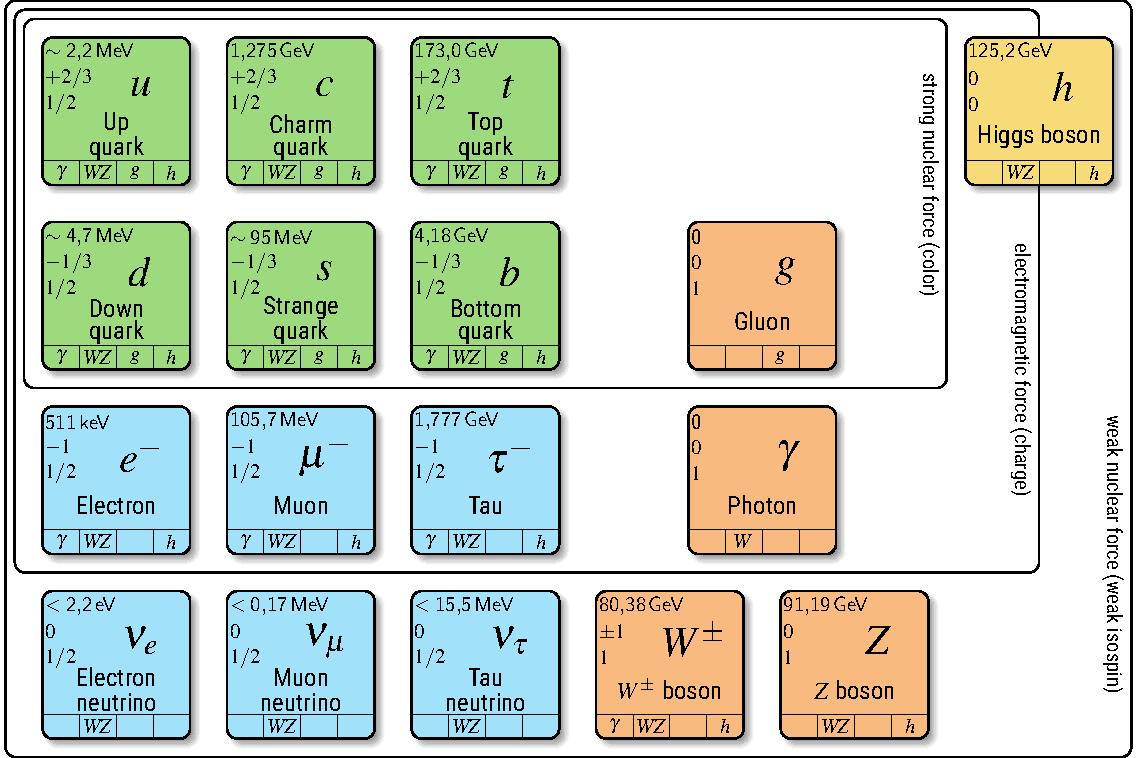
\includegraphics[scale=.575]{/home/torterotot/Documents/PhD-Thesis/tex/slides/SM_MSSM_HTT_pheno/SM_and_its_limits/SM_2018-bak.pdf}
}
\end{center}
\end{frame}

\begin{frame}
\frametitle{The Standard Model and its limits}
%pas de gravitation, déséquilibre matière/antimatière, matière noire, masses des neutrinos.
%Ce modèle ne rend cependant pas
%compte de nombreuses observations expérimentales, telles l’existence de la matière et
%de l’énergie noire et l’asymétrie entre matière et antimatière, et est généralement consi-
%déré comme une théorie effective de basse énergie d’une théorie plus fondamentale.
%De nombreuses théories au-delà du Modèle Standard ont été proposées mais aucune
%n’a encore été confirmée.

\begin{center}\Large
\begin{tikzpicture}[scale=2]
\draw (0,0) node {gravity?};
\draw (1.5,1) node {matter vs antimatter?};
\draw (-2,.25) node {dark matter?};
\draw (-1.5,-.75) node {dark energy?};
\draw (2,-1.5) node {neutrinos masses?};
\end{tikzpicture}
\end{center}

\end{frame}
